\documentclass[a4paper,12pt,times,numbered,print,index]{report}
\usepackage{vntex}
\usepackage{graphicx}
\usepackage{tabularx, caption}
\usepackage{amsmath}
\usepackage{array}
\usepackage{pdfpages}
\usepackage[pdftex]{hyperref}
\usepackage[toc]{appendix}
\usepackage{tabularx, makecell, multirow}
\usepackage{float}
\usepackage{color,soul}
\usepackage{listings}

\title{BÁO CÁO THỰC TẬP TỐT NGHIỆP}

\usepackage{indentfirst}

\definecolor{dkgreen}{rgb}{0,0.6,0}
\definecolor{gray}{rgb}{0.5,0.5,0.5}
\definecolor{mauve}{rgb}{0.58,0,0.82}

\lstdefinelanguage{JavaScript}{
	keywords={typeof, new, true, false, catch, function, return, null, catch, switch, var, if, in, while, do, else, case, break},
	keywordstyle=\color{blue}\bfseries,
	ndkeywords={class, export, boolean, throw, implements, import, this},
	ndkeywordstyle=\color{darkgray}\bfseries,
	identifierstyle=\color{black},
	sensitive=false,
	comment=[l]{//},
	morecomment=[s]{/*}{*/},
	commentstyle=\color{purple}\ttfamily,
	stringstyle=\color{red}\ttfamily,
	morestring=[b]',
	morestring=[b]"
}

\lstset{
	language=JavaScript,
	backgroundcolor=\color{white},
	extendedchars=true,
	basicstyle=\footnotesize\ttfamily,
	showstringspaces=false,
	showspaces=false,
	numbers=left,
	numberstyle=\footnotesize,
	numbersep=9pt,
	tabsize=2,
	breaklines=true,
	showtabs=false,
	captionpos=b
}

\begin{document}
	\begin{center}
		{ ĐẠI HỌC QUỐC GIA THÀNH PHỐ HỒ CHÍ MINH \\
			TRƯỜNG ĐẠI HỌC BÁCH KHOA \\
			KHOA KHOA HỌC VÀ KỸ THUẬT MÁY TÍNH} 
		\\
		\bigskip
		\bigskip
		\bigskip
		
\includegraphics[scale=.4]{Graphics/bachkhoa_logo}\\
		\bigskip
		\bigskip
		\bigskip
		LUẬN VĂN TỐT NGHIỆP ĐẠI HỌC \\
		\bigskip
		{\Huge \textbf{Giải pháp Thương mại điện tử trong Mạng xã hội và hiện thực}}
		\bigskip

		
		\begin{table}[h]
			
			\begin{tabular}{rll}
				\hspace{5 cm}  Hội đồng 3: & Hệ thống và Mạng máy tính \\
				\hspace{5 cm}  GVHD: & TS. Nguyễn Đức Thái \\
				\\
				 Thực hiện: \\
				Sinh viên thực hiện 1& Phạm Phương Uyên & 51204447 \\
				Sinh viên thực hiện 2 & Nguyễn Chí Thanh & 51203336 \\
			\end{tabular}
		\end{table}
		\vspace*{\fill}
		{\footnotesize TP. HỒ CHÍ MINH, THÁNG 12/2016}
	\end{center}
	\thispagestyle{empty}
	
	\newpage
	\pagenumbering{arabic}
		
	\renewcommand{\abstractname}{Lời cảm ơn}
	\begin{abstract}
		Xin chân thành cảm ơn sự hướng dẫn tận tình của thầy Nguyễn Đức Thái, CNBM Hệ thống \& Mạng Máy tính, khoa Khoa học và Kỹ thuật Máy tính, trường Đại học Bách Khoa TP.HCM đã luôn theo dõi, hướng dẫn chúng tôi tận tình trong quá trình thực hiện đề tài này.
		
		Để hoàn thành đề tài này, chúng tôi đã nhận được không ít sự hỗ trợ và những ý kiến đóng góp cả về kiến thức, công cụ và tinh thần từ các anh chị đi trước và các bạn...................
		
		Chúng tôi cũng xin chân thành cảm ơn tác giả của các tài liệu, bài viết mà chúng tôi đã tham khảo được liệt kê ở cuối tài liệu này.
		\flushright TP HCM, tháng 12 năm 2016\\
		\flushright Nhóm thực hiện
		
	\end{abstract}
	
	\renewcommand{\aa}{Lời cam đoan}
	\begin{center}
		\textbf{Lời cam đoan}
		............................
	\end{center}

	\renewcommand{\abstractname}{Tóm tắt nội dung}
	\begin{abstract}
		Mạng xã hội và Thương mại điện tử là hai khái niệm không còn xa lạ với tất cả những người sử dụng Internet hiện nay, nhưng độ phổ biến của chúng và mức độ quan tâm của người dùng Internet đối với chúng chưa bao giờ suy giảm. Hai khái niệm này đang có sự giao thoa đáng kể trong thời kỳ truyền thông xã hội phát triển mạnh mẽ và các bạn trẻ khởi nghiệp kinh doanh thành phong trào như hiện nay.
		
		Trong luận văn này chúng tôi đề xuất một giải pháp ít nhiều có tính khả thi để kết hợp hai khái niệm trên một cách chặt chẽ và hiện thực trực quan chúng trên một mạng xã hội nhỏ đơn giản, hệ thống bao gồm:
		\begin{itemize}
			\item Mạng xã hội với các yếu tố định nghĩa nó: các mối quan hệ xã hội và các tương tác xã hội;
			\item Sàn thương mại điện tử với nhiều chức năng phổ biến của thương mại điện tử, đây là một phần của mạng xã hội với nội dung chia sẻ là hàng hoá cần bán;
			\item Các chức năng hỗ trợ giao dịch;
			\item Các chức năng hỗ trợ quản lý sàn giao dịch và thu lợi từ website;
			\item Admin dashboard cho người quản trị mạng xã hội và quản lý sàn thương mại.
		\end{itemize}
		
		Hệ thống này khi hoàn thiện hoàn toàn có khả năng được đưa vào sử dụng trong thực tế như một mạng xã hội kinh doanh, khả năng mở rộng của nó là vô hạn.
	\end{abstract}
		
	\tableofcontents
	\listoffigures
	\listoftables
	
	\chapter{Giới thiệu}
\section{Giới thiệu về đề tài, thực trạng và lý do chọn đề tài}
Mạng xã hội và Thương mại điện tử là hai khái niệm không còn xa lạ với tất cả những người sử dụng Internet hiện nay, nhưng độ phổ biến của chúng và mức độ quan tâm của người dùng Internet đối với chúng chưa bao giờ suy giảm. 

Gần đây, các mạng xã hội lớn như Facebook, Twitter, Instagram, LinkIn, Google+ đang đều đang từng bước hiện thực các giải pháp hỗ trợ người dùng kinh doanh ngay trên mạng xã hội của họ, chính sách này hứa hẹn một nguồn thu khổng lồ bởi vì mạng xã hội là nơi có sức hấp dẫn rất lớn đối với không chỉ các nhà bán lẻ (bất cứ người dùng mạng xã hội nào cũng có tiềm năng trở thành một nhà bán lẻ!) mà còn các nhà buôn, các doanh nghiệp sản xuất hàng hoá... Đây cũng là một mảnh đất giàu tiềm năng của truyền thông kỹ thuật số. Tuy nhiên, nhóm nhận xét rằng việc tích hợp Thương mại điện tử trong Mạng xã hội hiện nay chỉ mới dừng lại ở phạm vi hiển thị, tức là, chưa có sự hỗ trợ của hệ thống mạng xã hội trong toàn bộ quá trình giao dịch. 
Với chiều ngược lại, các trang thương mại điện tử hiện nay cũng đang có xu hướng tăng cường sự gắn kết và khả năng tương tác giữa các bên tham gia trao đổi hàng hoá, chẳng hạn, các trang bán lẻ quy mô lớn hiện nay đều tích hợp tính năng gửi thư điện tử (email), trò chuyện trực tuyến (chat) và hệ thống thảo luận, phê bình nhận xét (review) và đánh giá (rating). Tuy nhiên, trên thực tế những chức năng này chỉ là tương tác nhị phân 2 chiều, chưa đủ nhanh nhạy và đáng tin để tương xứng với một thời kỳ mà truyền thông xã hội chiếm một vai trò rất quan trọng như hiện nay.

Vì thế, trong luận văn này nhóm em đề xuất một giải pháp ít nhiều có tính khả thi để kết hợp hai khái niệm trên và hiện thực trực quan chúng trên một mạng xã hội nhỏ đơn giản, hệ thống bao gồm:

\section{Mục tiêu đề tài}
Mục tiêu đề tài là nghiên cứu đặc điểm của mạng xã hội trực tuyến và thương mại điện tử, phân tích mối liên hệ giữa hai vấn đề này, đề xuất một hình kết hợp giữa hai khái niệm, qua đó phân tích ưu nhược điểm của sự kết hợp, khả năng ứng dụng trong thực tiễn cũng như khả năng mở rộng và sinh lợi từ mô hình, cuối cùng hiện thực mô hình website hoàn chỉnh.

\section{Nội dung đề tài}
Đề tài \"Giải pháp thương mại điện tử trong mạng xã hội\", bao gồm 2 nội dung chính sau:
\begin{itemize}
	\item Nghiên cứu hiện tượng mạng xã hội trực tuyến
	\item Nghiên cứu các giải pháp thương mại điện tử
	\item Đề xuất một giải pháp thương mại điện tử trong mạng xã hội cùng với ưu, nhược điểm của nó, khả năng mở rộng cũng như sinh lợi của mô hình này
	\item Hiện thực giải pháp
\end{itemize}

\section{Giới hạn đề tài}
\begin{enumerate}
	\item Đề tài là "Giải pháp Thương mại điện tử trong Mạng xã hội" nên chúng tôi tập trung vào vấn đề tích hợp thương mại điện tử trong mạng xã hội chứ không đặt trọng tâm tạo ra mạng xã hội, khi hiện thực chúng tôi sử dụng một Social Networking CMS có sẵn để hiện thực giải pháp trên đó.
	
	\item Thương mại điện tử là một lĩnh vực rộng lớn bao gồm nhiều hình thái và phạm trù khác nhau, nên trong luận văn này, mô hình của chúng tôi dừng lại ở mức tập trung và hỗ trợ tốt nhất cho hình thức thương mại điện tử Business-to-Custommer (B2C), Customer-to-Customer (C2C) và hướng tới những người có nhu cầu bán lẻ hàng tiêu dùng.
	
	\item Mô hình đề xuất bao gồm cả quá trình thanh toán với nhiều sự lựa chọn phương thức thanh toán khác nhau nhưng trong việc hiện thực bản thử nghiệm chúng tôi ssẽ chỉ trình bày mẫu một cổng thanh toán mà thôi.
	
	\item .............
\end{enumerate}

\section{Cấu trúc luận văn}
\textit{Chương 1:} Giới thiệu

Giới thiệu đề tài, thực trạng và lý do chọn đề tài; giới thiệu mục tiêu và phạm vi của đề tài; nội dung đề tài và cấu trúc của luận văn.

\textit{Chương 2:} Các hệ thống liên quan trong thực tế

Giới thiệu minh hoạ một số hệ thống đang tồn tại hoạt động trong các lĩnh vực liên quan; phân tích và so sánh.

\textit{Chương 3:} Các kiến thức và công nghệ nền

Đúc kết các nghiên cứu về đặc điểm mạng xã hôi, đặc điểm của thương mại điện tử và tiềm năng kết hợp chúng. Giới thiệu các công cụ và kiến thức sử dụng để thực hiện.

\textit{Chương 4:} Mô hình đề xuất cho giải pháp thương mại điện tử trong mạng xã hội

Trình bày chi tiết mô hình website đề xuất.

\textit{Chương 5:} Hiện thực mô hình đề xuất

Trình bày chi tiết kỹ thuật trong việc hiện thực mô hình website.

\textit{Chương 6:} Đánh giá mô hình đề xuất

...

\textit{Chương 7:} Đánh giá kết quả thực hiện

...

\textit{Chương 8:} Kết luận

...


	\chapter{Các hệ thống liên quan trong thực tế}

\section{Các nhà cung cấp dịch vụ Mạng xã hội và truyền thông xã hội đang từng bước hỗ trợ kinh doanh trực tuyến}
\subsection{Facebook với Shopping Marketplace}

Facebook là mạng xã hội rất phổ biến, cho phép người dùng đăng tải ảnh, video, chia sẻ những status cảm xúc, gửi các thông điệp tới bạn bè. Tuy nhiên trong những năm gần đây nhiều người đã sử dụng Facebook để kết nối theo cách khác: mua và bán. Hoạt động này bắt đầu trong Facebook Groups và đã phát triển đáng kể. Hơn 450 triệu người đến tham quan mua và bán các nhóm mỗi tháng - từ các gia đình trong một khu phố địa phương cho tới quy mô toàn thế giới.

\begin{figure}[H]
	\centering
	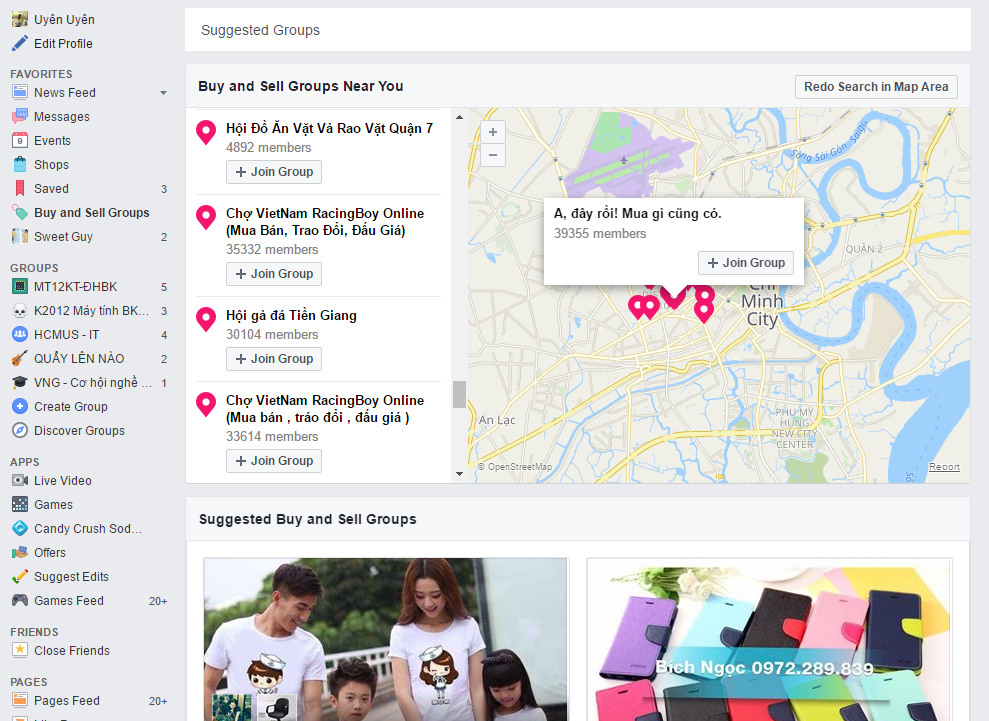
\includegraphics[scale=.5]{img/fb-group-buy.PNG} 
	\caption{Facebook Groups - Buy and Sell Groups}
\end{figure}

Nhằm hỗ trợ cho sự tương tác mới này, Facebook đã cho ra đời Facebook Marketplace, nơi người dùng có thể lên danh sách những thứ họ có hoặc mong muốn trong một phạm vi kết nối ("[...] to list what you have and what you want within your group of friends, networks, or other networks. Beyond its use for classified listings, you can use Marketplace to get a sense of everything available or desired within your networks."\cite{facebooknote1}).

Một số hình ảnh của Facebook Marketplace:

\begin{figure}[H]
	\centering
	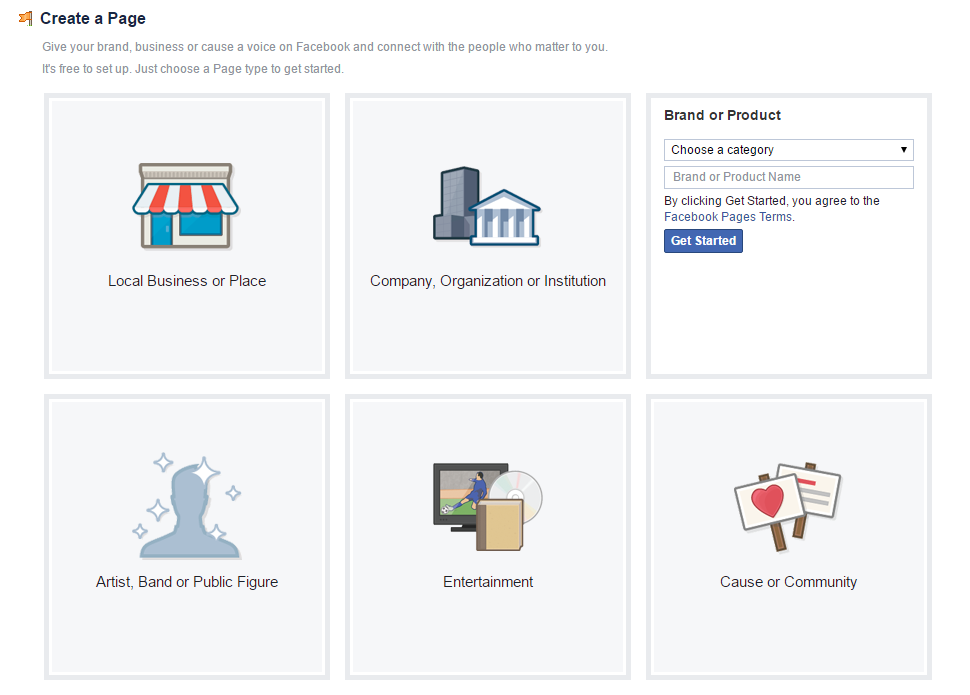
\includegraphics[scale=.5]{img/fb-create-page.PNG} 
	\caption{Tạo một Page trong Facebook Marketplace}
\end{figure}

\begin{figure}[H]
	\centering
	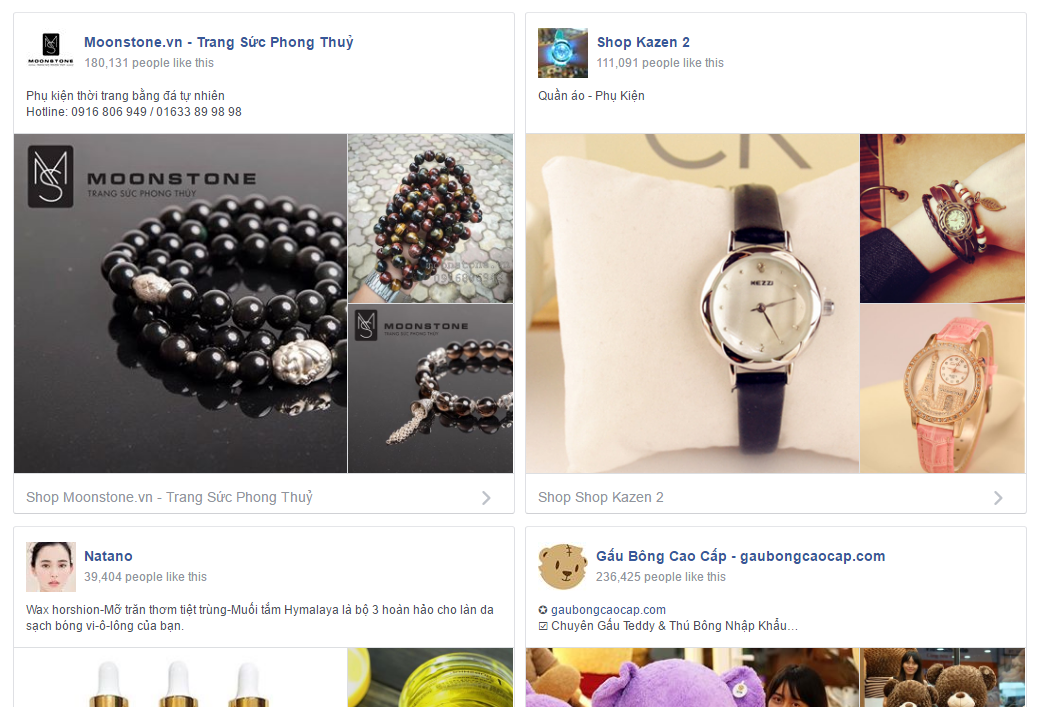
\includegraphics[scale=.5]{img/fb-shop.PNG} 
	\caption{Các Pages được trình bày tại trang chính của Marketplace}
\end{figure}

\begin{figure}[H]
	\centering
	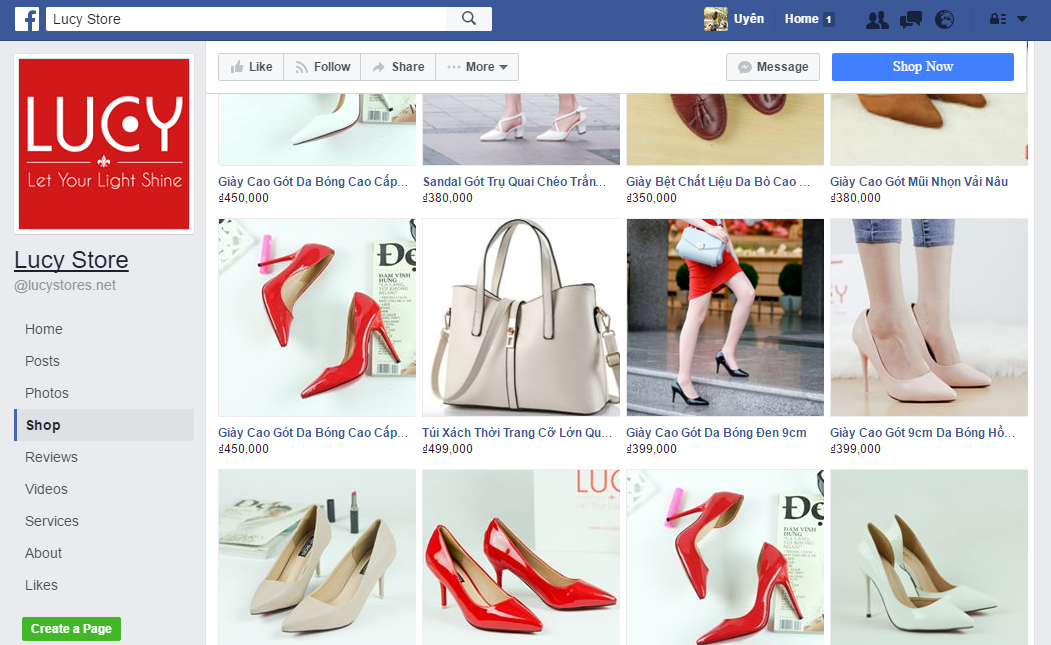
\includegraphics[scale=.5]{img/fb-in-store.PNG} 
	\caption{Giao diện trong Page được thiết kế như một cửa hàng trực tuyến}
\end{figure}

Từ những thông tin trên, ta thấy mạng xã hội này đang từng bước đưa khái niệm thương mại điện tử vào trong hệ thống của họ. Tuy nhiên, việc mua bán này chỉ đang dừng lại ở mức độ giao diện, trưng bày chứ chưa hỗ trợ người dùng trong toàn bộ quá trình mua, bán.

\subsection{Pinterest với "Buyable Pins"}
Khởi đầu với một trang web chia sẻ hình ảnh trực tuyến được biết đến như là "danh mục ý tưỏng" ("catalog of ideas" - CEO Ben Silbermann) hơn là một mạng xã hội. Tuy nhiên, vào tháng 6/2015 Pinterest tuyên bố phát hành những "Buyable Pins", là những "Pin" được tích hợp nút "Buy it" bên cạnh nút "Pin it" thông thường. Những "Pin" này được tạo bởi các doanh nghiệp để quảng bá sản phẩm của họ thông qua Pinboards. Người dùng cũng có thể thấy giá của các mặt hàng, và được hỗ trợ để thanh toán (mua) ngay trên Pinterest thông qua Apple Pay hoặc Credit Cart. 

\begin{figure}[H]
	\centering
	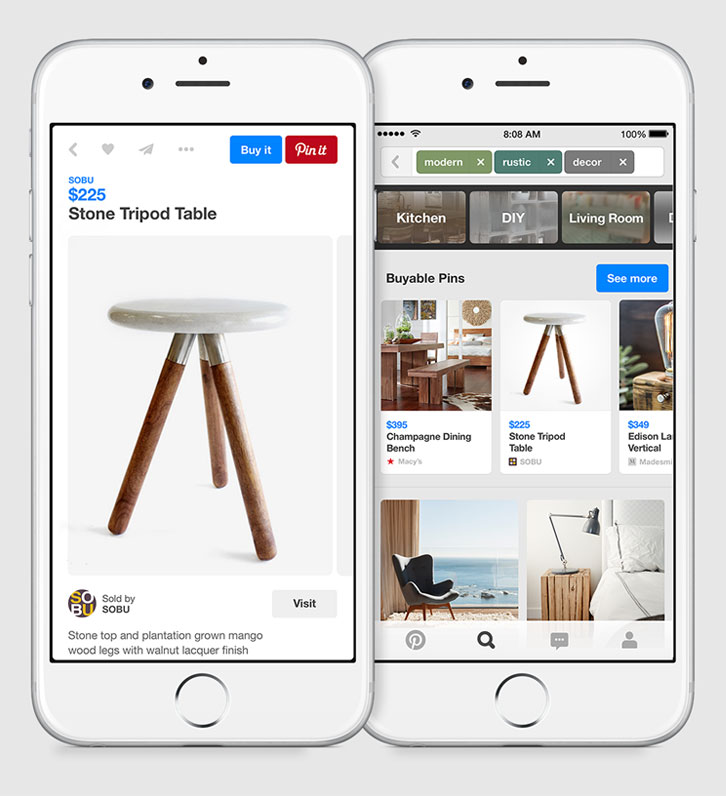
\includegraphics[scale=.4]{img/pin-buypins.jpg} 
	\caption{Buyable pins trên Iphone}
\end{figure}

Với lợi thế về khả năng chia sẻ của Pinterest, khi người mua "re-pin" một thứ mà họ thích, nó sẽ được lan truyền và tiếp thị rộng rãi như virus, lan sang các nhóm khác nhau. 

Dù được quảng cáo với nhiều ưu điểm tuyệt vời, mua bán trên Pinterest vẫn còn những hạn chế. Những người chủ của Pinterest không muốn sản phẩm của mình là một mạng xã hội mà quyết giữ nó theo quan điểm ban đầu và luôn duy trì quan điểm thận trọng đối với sự phát triển mới\cite{AllYouNeedtoKnowAboutPinterestBuyablePins}, hiện tại khả năng mua bán của nó có được là do sự liên kết với những nền tảng thương mại điện tử khác một cách hạn chế bao gồm BigCommerce, Demandware, Magento và Shopify, và hiện chỉ hoạt động tại Mỹ. Do đó, việc mua bán và thanh toán trên Pinterest gặp nhiều khó khăn.

(lợi thế của sự hợp tác giữa shopify với pinterest)

(nhận xét chung)
\section{Các trang thương mại điện tử đang từng bước cải thiện sự tương tác thành viên}

\subsection{Chợ điện tử Alibaba với }

\subsection{Amazon}

Mục đích của việc tích hợp tính năng xã hội trong các ứng dụng thương mại điện tử là để động viên người tiêu dùng truy cập ứng dụng thường xuyên hơn và trong thời gian dài của thời gian, với hy vọng chuyển đổi lần vào bán hàng.


	\chapter{Các kiến thức và công nghệ nền}

\section{Các khái niệm và kiến thức liên quan}

\section{Các công nghệ nền và kỹ thuật sử dụng}
(...)
\subsection{Zend Framework}
\subsubsection{Tổng quan}

Zend Framework là một framework mã nguồn mở được sử dụng để phát triển các ứng dụng web và các dịch vụ với PHP 5. Zend Framework được hiện thực 100\% code hướng đối tượng. Cấu trúc của các thành phần Zend framework có tính độc đáo; mỗi thành phần được thiết kế với ít phụ thuộc vào các thành phần khác. kiến trúc lỏng lẻo này cho phép các nhà phát triển có thể sử dụng thành phần riêng tùy theo mục đích. Chúng ta thường gọi là thiết kế "use-at-will".

Trong khi chúng có thể được sử dụng riêng rẽ, các thành phần của Zend Framework trong thư viện chuẩn tạo thành một khung ứng dụng web mạnh mẽ và mở rộng khi kết hợp. Zend Framework cung cấp mạnh mẽ, hiệu suất cao cho việc hiện thực MVC, một cơ sở dữ liệu trừu tượng đó là đơn giản để sử dụng, và một thành phần hình thức mà thực hiện dưới dạng HTML rendering, validation, và filter để phát triển có thể củng cố tất cả các hoạt động sử dụng một dễ sử dụng , giao diện hướng đối tượng. Các thành phần khác, chẳng hạn như Zend\_Auth và Zend\_Acl, cung cấp cho người dùng xác thực và phân quyền chống lại tất cả các cửa hàng chứng chỉ. Dù nhu cầu ứng dụng của bạn, bạn có khả thể tìm thấy một thành phần Zend Framework có thể được sử dụng để làm giảm đáng kể thời gian phát triển với một nền tảng được kiểm tra một cách kỹ lưỡng.

Các nhà tài trợ chính của dự án Zend Framework là »Zend Technologies, nhưng nhiều công ty đã góp phần thành phần hoặc các tính năng đáng kể cho khuôn khổ. Các công ty như Google, Microsoft, và StrikeIron đã hợp tác với Zend để cung cấp giao diện với các dịch vụ web và các công nghệ khác mà họ muốn làm cho có sẵn cho các nhà phát triển Zend Framework.

Zend Framework có một cộng đồng phát triển và hỗ trợ tương đối lớn. Nơi mà chúng ta có thể trao đổi thông tin và chia sẻ những dự án lớn. Hỗ trợ rất nhiều cho việc lập trình.

\subsubsection{Mô hình MVC trong Zend Framework}
(...)

\section{Social Engine}
\subsubsection{Tổng quan}
SocialEngine PHP là một mạng xã hội thuần được viết dựa trên PHP, cung cấp các tính năng tương tự như một mạng xã hội trên trang web của người dùng. Các tính năng chính bao gồm quản trị mạng xã hội quy mô nhỏ đến trung bình, một số khả năng tuỳ biến, mã không mã hóa, khả năng đa ngôn ngữ, và khả năng tương thích tiện ích / phụ tùng mô-đun. Có một loạt các mẫu và các tiện ích có sẵn để mở rộng các tính năng cơ bản đã có trong lõi SocialEngine.

\subsubsection{Những ưu điểm khi chọn SocialEngine}
\begin{itemize}
	\item Quick Setup: Bạn có thể bắt đầu một trang web được thiết lập trong vài phút. Dễ dàng tích hợp vào trang web hiện tại của bạn.
	\item Social and friendly - có thể đăng nhập ngay lập tức với các tài khoản xã hội đang tồn tại của họ như twitter, Facebook vv Họ cũng có thể đăng tải các hình ảnh vv trở lại trên tài khoản của họ.
	\item Easily customizable- Nó rất dễ dàng để tùy chỉnh và có toàn quyền kiểm soát. Bất cứ ai cũng có thể thêm logo của riêng mình, hình ảnh, màu sắc, hình nền bố trí vv Và quá trình này không phải là phức tạp cả. Điều đó rất dễ dàng để xử lý và giải quyết.
	\item Individual Plugins - Và một trong những lợi ích tốt nhất của việc sử dụng nền tảng này là bạn không cần phải mua tiện ích trong một gói hoàn chỉnh. Bạn chỉ phải mua tiện ích mà cần thiết cho bạn không giống như các trang web khác. Tuy nhiên, bạn có thể thêm bất kỳ tiện ích khi bạn cảm thấy như nó được, hoặc bạn có thể tự tạo một tiện ích riêng cho chính website của bạn.
	\item Flexibility - SocialEngine cung cấp cho bạn một loạt các phong cách khác nhau, và bạn luôn có thể quyết định cách thành viên của bạn sẽ kết nối và tương tác với nhau. Nó có nhiều tùy chọn liên quan đến khuôn khổ xã hội với một kéo dễ dàng và thả trong quản lý. Nó cũng cung cấp cho bạn để có nhiều giai đoạn của thành viên, không có hạn chế.
	\item Active Support Team - Nhóm phát triển của SocialEngine là 100\% hoạt động với văn phòng ở Los Angeles, California của họ. Họ rất thân thiện và nhanh chóng. Bạn luôn có thể liên hệ với họ và nó chỉ là một cú nhấn chuột.
	\item Security - Hệ thống bảo mật trên nền tảng này là khá chặt chẽ và hữu ích quá. Họ có các tính năng bảo mật như cấm, ngăn chặn hoặc danh sách đen những lời lăng mạ và người sử dụng trái phép, nếu cần thiết. Ngoài ra còn có nhiều tùy chọn để kiểm soát các kẻ gửi thư rác bằng tay.
	\item Non encrypted plugins and source code - Mã nguồn không được mã hóa để bất cứ ai có thể thay đổi cách làm việc một phần mềm đặc biệt. Nhiều tiện ích được tính phí, nhưng chủ yếu là các tiện ích cộng đồng được miễn phí.
	\item Client showcase - Nó có một tính năng tuyệt vời như giới thiệu khách hàng, nơi bạn có thể tìm hiểu những gì người khác khách hàng đã tạo ra sử dụng nền tảng này.
	Language packs - SocialEngine có một lượng lớn các gói ngôn ngữ khác nhau, ví dụ Pháp, Tây Ban Nha, vv
	\item Activity feed - Nó có một activity feed. Trong activity feed, các thành viên có thể xem bài của nhau mà họ đang theo dõi hoặc đang trong danh sách bạn bè của họ. Khái niệm thức activity feed này khá giống với các nguồn tin của Facebook hoặc Google plus. Tại đây, người ta cũng có thể lọc bài dựa trên sở thích.
	\item Private Messages- Các tin nhắn riêng tư cho phép người sử dụng để liên lạc với các thành viên cá nhân, giống như bất kỳ nền tảng xã hội khác như Facebook hay Google plus. Bất cứ ai cũng có thể gửi tin nhắn cho nhiều người cùng một lúc.
\end{itemize}

\subsubsection{Kết luận}
SocialEngine chắc chắn là một phương tiện hiệu quả cho những ai đang săn cứng cho một phần mềm mạng xã hội chất lượng phong phú, đáng tin cậy, và khách hàng quen. Công cụ này có thể là lựa chọn hoàn hảo của bạn trong trường hợp bạn cần giám định lập trình. Trong trường hợp bạn đang ở trên một ngân sách chặt chẽ, bạn có thể sử dụng tùy chọn của nó miễn phí quá. Một số khách hàng đã tìm thấy này chậm để tải và áp dụng và nói khi họ thêm rất nhiều plugin nó làm chậm toàn bộ điều xuống, nhưng SocialEngine.com trả lời nói rằng họ đã cảnh báo về "một số vấn đề" và đang làm việc để giải quyết chúng.
	\chapter{Mô hình đề xuất cho giải pháp thương mại điện tử trong mạng xã hội}

\section{Mạng xã hội trực tuyến}

	\chapter{Hiện thực mô hình đề xuất}
	\chapter{Đánh giá mô hình đề xuất}
\section{Khả năng giải quyết bài toán đặt ra}
\section{Tính ứng dụng của mô hình}
\section{Khả năng mở rộng của mô hình}
\section{Tính khả thi của mô hình}
	\chapter{Đánh giá kết quả hiện thực}
\section{Kiểm thử hệ thống phần mềm}
	\chapter{Kết luận}

		
	\bibliographystyle{plain}
	\bibliography{ref}
	

		
\end{document}
